\chapter{Appendix}
\section{Getting started with JSBML}
The most important thing to know about JSBML is that this library mostly is a literal implementation of the SBML-structures defined in the SBML specifications \cite{hucka2018systems} \cite{sbmlqual2015}. The JSBML-classes represent the structures defined in SBML, providing getter- and setter methods to populate their fields.

In figure \ref{fig:JSBMLSpecies} the steps required from reading an SBML-file to the extraction of an SBML-qual model's species are shown. After specifying the path to the SBML-file to be read, JSBML's \emph{SBMLReader} is used to read the provided file. This returns an object of type \emph{SBase}, an abstract class used for all SBML-object types, that stores meta-data about the object, such a the SBML-level and version used to represent it. To gain access to the SBML-file data representation, it need to be cast to the \emph{SBMLDocument}-type used to represent SBML-files. The \emph{Model} it contains can the be retrieved by calling the \texttt{getModel()}-method.

Model represented by one of the SBML-extensions are not represented by the \emph{Model}-class itself, but instead by a separate model-class. In case of SBML-qual, this is the \emph{QualModelPlugin-class}, which can be retrieve from the main \emph{Model} by calling the \texttt{getExtension()}-method using "qual" as an key to the extension map. In the last step of the figure, the species are then retrieved using the appropriate getter-method.

Retrieving SBML-transitions an the structures contained within, works in the same manner as with species and the other SBML-structures, which is why these are not included as a demo in this report. However, the \emph{JSBMLReadingDemo}-class in the \emph{sbml.demos} package in the repository contains a full demo of the code used to read the various SBML structures required by the converter.

\begin{figure}[H]
    \centering
    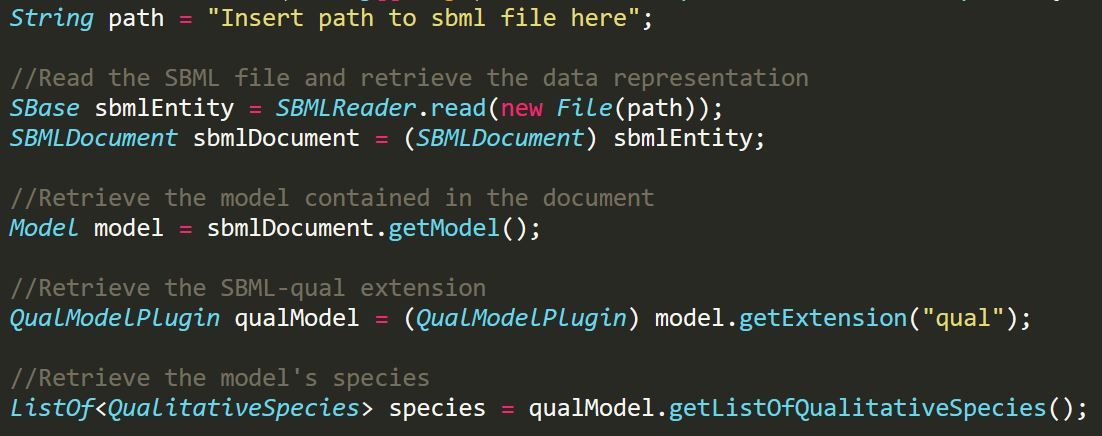
\includegraphics[scale=0.60]{Sections/Images/JSBMLSpecies.JPG}
    \caption{Species retrieval using JSBML}
    \label{fig:JSBMLSpecies}
\end{figure}

When creating object to represent SBML-structures is very important to use a consistent SBML-level and version for all object in a model representation, as JSBML will complain and throw exceptions otherwise. While almost all SBML-structures have default constructors that allow their creation without specifying level and version, it is a good idea to specify them anyway, as unset version also can cause several problems. In the converter's implementation this problem has been solved by adding a \emph{configuration}-package, which is used to set SBML-level and version for the entire converter.

In figure \ref{fig:JSBMLCreation}, it is shown how to create a small (and empty) SBML-model with an SBML-qual extension. Using either \emph{set}- or \emph{add}-methods, the various structures are added to their parents. When dealing with instances of the \emph{ListOf<>}-structure it is important to the parent of those lists to be the \emph{Model}, they are contained in. If this is not done, JSBML will not recognize these lists as part of the model and throw an exception. 

\begin{figure}[H]
    \centering
    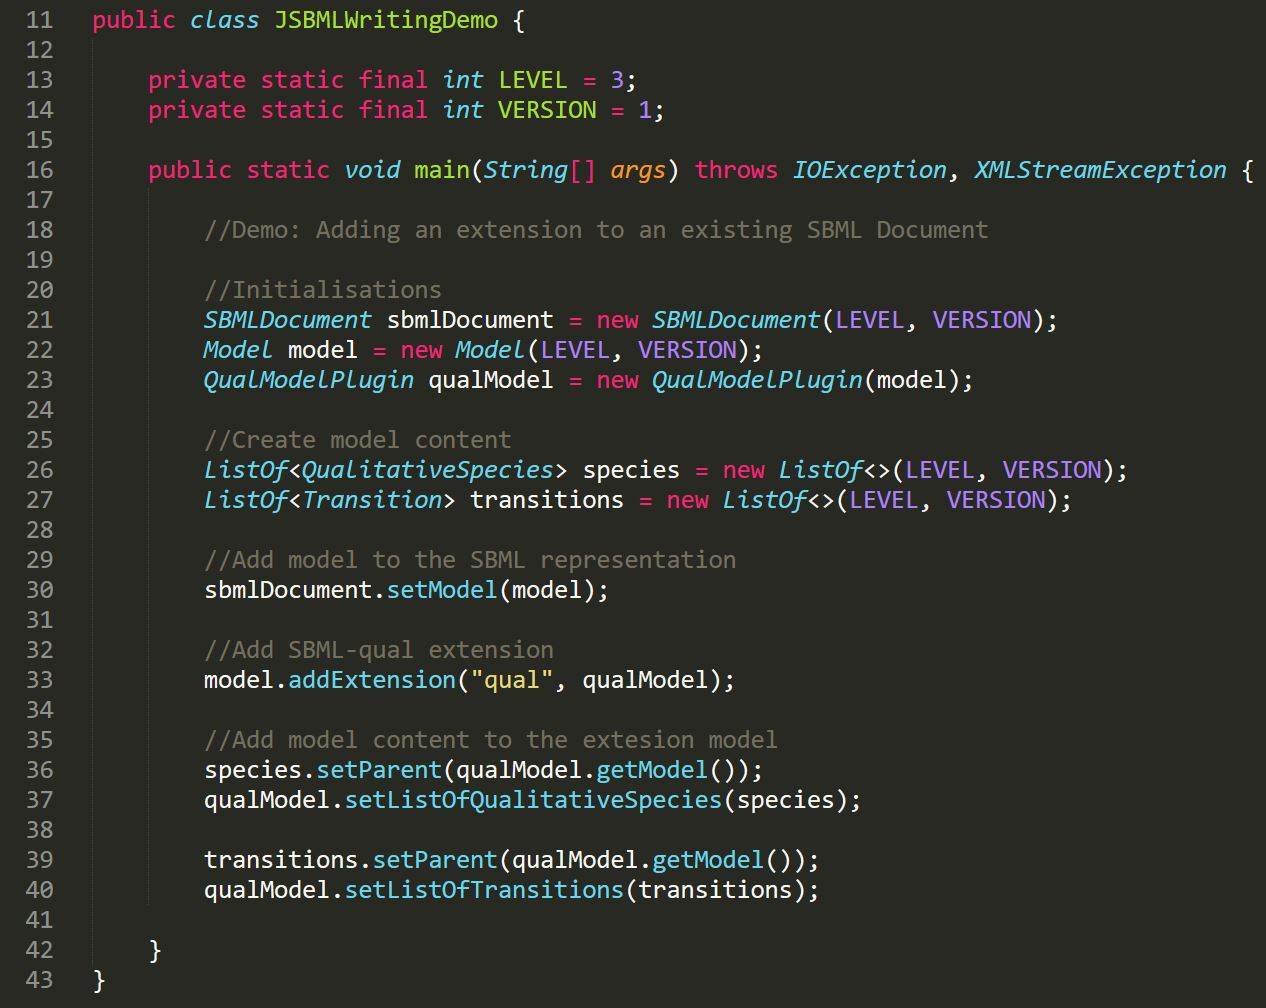
\includegraphics[scale=0.50]{Sections/Images/JSBMLCreation.JPG}
    \caption{SBML model generation using JSBML}
    \label{fig:JSBMLCreation}
\end{figure}

When dealing with the JSBML-functionality used in the converter, the last important part is to know how to create the logical expressions in the \emph{FunctionTerm}-structures used by SBML. For this, the \emph{ASTNode}-class is used, which represents the MathML-elements of an SBML-file.

 \ref{fig:ASTNode} shows the most important ways to construct \emph{ASTNodes} in this converter. Depending on what input is given to the constructor, the \emph{ASTNode} will represent a different element. As shown in the figure, variables can be create by providing the variable name in form of a string. Integer constants on the other hand are created by providing an integer value. To create other types, such as Boolean constants and operator, the \emph{ASTNode}-class also provides the \emph{Type}-enum, which defines all operators and special constants \emph{ASTNodes} can represent. The other figure (\ref{fig:ASTNode}) shows how to initialise and retrieve data from an AST consisting of \emph{ASTNode}-objects.

\begin{figure}[H]
    \centering
    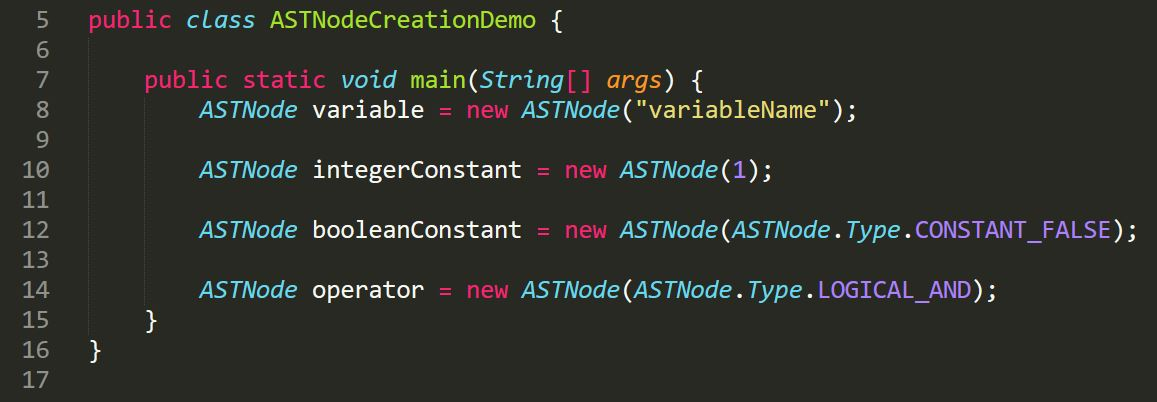
\includegraphics[scale=0.55]{Sections/Images/ASTNodes.JPG}
    \caption{Examples of ASTNodes representing elements of an AST}
    \label{fig:ASTNode}
\end{figure}

\begin{figure}[H]
    \centering
    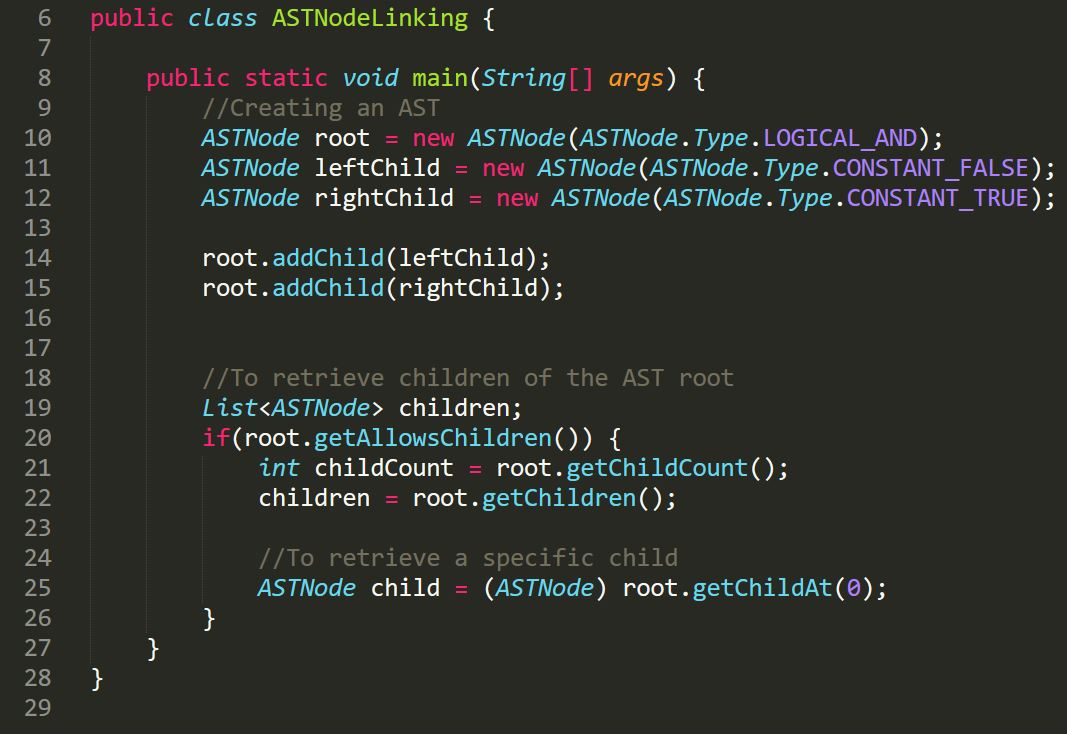
\includegraphics[scale=0.6]{Sections/Images/ASTLinking.JPG}
    \caption{Example of an AST initialisation and data retrieval from it}
    \label{fig:ASTLinking}
\end{figure}

\section{Extending the converter to support MNs}
To add support for multi-valued models in the converter only requires minor changes to the existing functionality. In total only four different methods need to be extended or modified.
Before explaining the required changes, it needs to be mentioned that the classes used to represent integer-values in ERODE, \textbf{must implement} the \emph{IUpdateFunction}-interface for this modification to work. Should this not be the case, the node conversion module in the \emph{sbml.conversion.nodes} package would need to be replaced by a different module that also implements the \emph{INodeConverter}-interface.

To extend the converter using the existing modules, the first method that needs to be modified, is the \texttt{create()}-method in the \emph{NodeManager}-class shown in figure \ref{fig:MNCreate}. This method analyzes the given update function element from ERODE's AST to analyze its type. Depending on its type, it then calls the corresponding manager to continue the converter initialisation. Since the missing update function type is a type representing integers, this is part of the \emph{ValueASTConverter}'s responsibilities.

The simplest way to modifiy is method is to move the \\
\texttt{return ValueASTConverter...} statement to the default case, replacing the current exception. Once that is done the \emph{REFERENCE},\emph{TRUE} and \emph{FALSE} cases can be removed. Since the exception in the default case currently only serves the purpose of catching the new update function type(s), once ERODE is extended it will no longer be needed.

\begin{figure}[H]
    \centering
    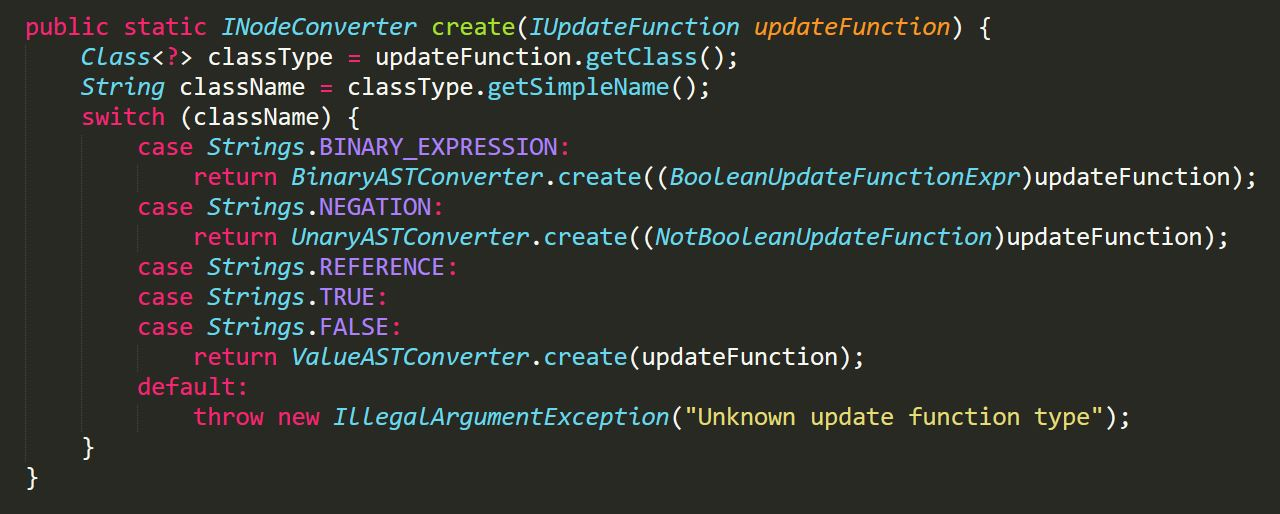
\includegraphics[scale=0.5]{Sections/Images/MNCreate.JPG}
    \caption{The \texttt{create()}-method used when converting to SBML}
    \label{fig:MNCreate}
\end{figure}

The next method to be changed, is the \emph{convert()}-method in the \emph{ValueWriter}-class. This method simply requires an additional case, to take the new update function type into account. The \emph{currentNode} for the new case should be set to the result of the \emph{element.constant()}-call.

\begin{figure}[H]
    \centering
    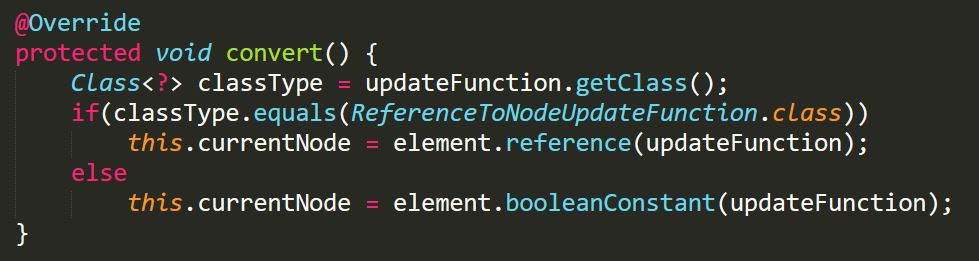
\includegraphics[scale=0.5]{Sections/Images/ValueWriterConvert.JPG}
    \caption{The \texttt{convert()}-method of the \emph{ValueWriter}-class}
    \label{fig:WriterConvert}
\end{figure}

Once these steps have been performed, the actual conversion step for the integer representations need to be implemented in the \emph{SBMLElement}-class. This class currently contains an unused method, called \texttt{constant()}, taking an \emph{IUpdateFunction}-instance as input and returns an \emph{ASTNode}, using the \emph{ASTNodeBuilder}.
The current method body, can be replaced entirely, since this method will take integer representations as input and not Boolean constants. The method body would then simply require some way of reading the \emph{IUpdateFunction}'s integer value and pass it to the \emph{ASTNodeBuilder}'s \texttt{integer()}-method, which creates integer constants.

\begin{figure}[H]
    \centering
    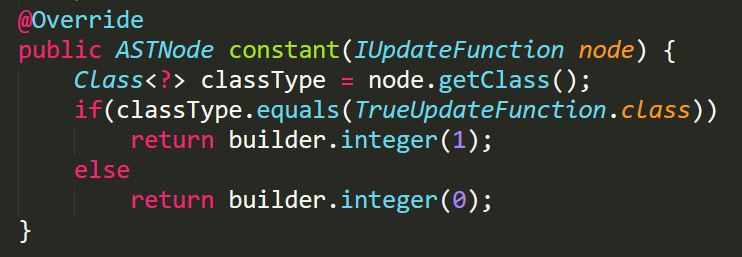
\includegraphics[scale=0.5]{Sections/Images/ConstantMethod.JPG}
    \caption{The current \texttt{constant()}-method in the \emph{SBMLElement}-class}
    \label{fig:SBMLconstant}
\end{figure}

Finally, the \texttt{constant()}-method, implemented by the \emph{ERODEElement}, also requires adjustment, since it currently translates SBML-integers to ERODE-booleans. The new version should return ERODE's integer-representation instead.

\begin{figure}[H]
    \centering
    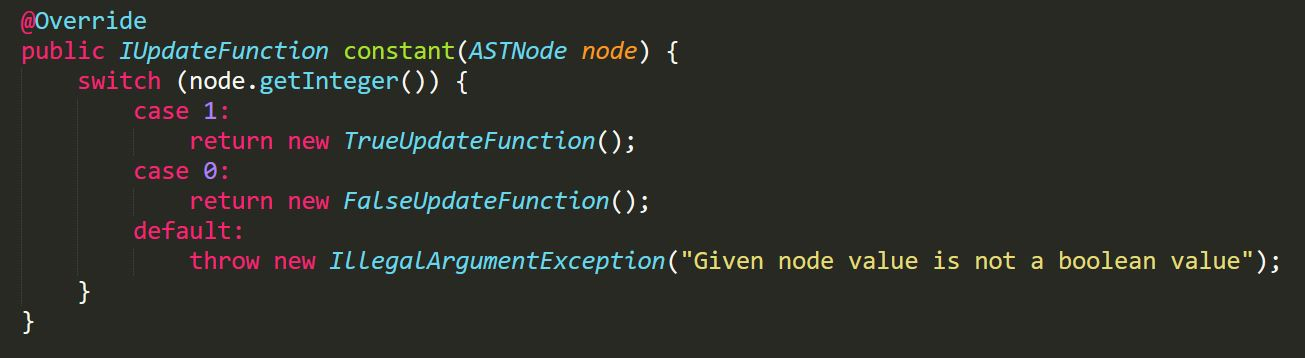
\includegraphics[scale=0.5]{Sections/Images/ERODEconstant.JPG}
    \caption{The current \texttt{constant()}-method in the \emph{ERODEElement}-class}
    \label{fig:ERODEconstant}
\end{figure}